\chapter{Basics}\label{ch:basics}
This chapter provides a collection of basic knowledge as a foundation for this work. It covers fundamental concepts and techniques essential for understanding the subsequent chapters.

\section{Real Time Operating Systems}\label{sec:rtos}
A \ac{RTOS} is designed with precise timing and high reliability in mind for running applications\cite{stankovicRealtimeOperatingSystems2004}. Such systems are used in a wide range of applications, from multimedia systems and smart home systems to automotive and medical sectors, such as pacemakers\cite{hambardeSurveyRealTime2014}. In all these systems, the correctness and timeliness of the applications are of utmost importance\cite{hambardeSurveyRealTime2014}.

\subsection{Tasks and Jobs}\label{sec:tasks_and_jobs}
According to the \textcite{IEEEStandardRealTime}, a task is defined as the ``basic logical unit of concurrent program execution'' that contains code. The standard also states that while the code within a task is executed sequentially, the tasks themselves may run in parallel with other tasks. Tasks can have deadlines based on their importance and the nature of their work. If a task misses its deadline due to insufficient computational time, the system and results may be affected differently. It is common to categorize task deadlines into three types\cite{dengSchedulingRealtimeApplications1997,abeniIntegratingMultimediaApplications1998,shindeComparisonRealTime2017}:
\begin{enumerate}
	\item \textbf{Hard Deadline:}
		  Missing a hard deadline is considered a system failure. The task must complete by its deadline; otherwise, the system may enter an unsafe state.
	\item \textbf{Firm Deadline:}
		  Missing a firm deadline does not cause a system failure, but the task's result is no longer useful and is discarded. The system continues to operate, but the quality of service may degrade.
	\item \textbf{Soft Deadline:}
		  Missing a soft deadline reduces the task's utility, but the result can still be used. The system can tolerate some deadline misses without significant impact on overall performance.
\end{enumerate}
A job is the specific execution instance of a given task when scheduled. One task may be assigned with multiple jobs. If a task is scheduled to execute every $x$ time units, the total number of jobs will be equal to the number of times $x$ fits within the inspection cycle. For a more comprehensive description on tasks and jobs, refer to \cref{sec:task}.

\subsection{Real-time Scheduling}\label{sec:scheduling}
Creating the schedule of given tasks to be executed some aspects

Generating a task set with known response times requires knowledge about the schedule. Implementing a scheduler gives the benefit of taking direct insights in the compilation of the generated results. 
When confronted with two or more tasks, the system needs to decide what task gets to be executed in the computational unit.
This is done by employing scheduling techniques, most rely on the use of priorities assigned to the tasks, others schedule the tasks purely on a timely basis.

\begin{itemize}
	\item \textbf{Clock based Scheduling:}
		With clock based scheduling every task gets a share of execution time in which the work of the task may be done. It is a way to schedule tasks without priorities whilst making sure every task gets time on the computational unit. While being a simple algorithm it does create a lot of overhead, since the timeslots do not necessarily encompass the whole time needed by the task.
	\item \textbf{(Weighted) Round Robin:}
		In basic Round Robin scheduling, each task is assigned a fixed time slice or quantum in a cyclic order, ensuring all tasks get an equal share of CPU time. Weighted Round Robin extends this by assigning different weights to tasks, allowing tasks with higher weights to receive more CPU time compared to tasks with lower weights. This provides a more flexible and efficient scheduling mechanism, especially for systems with tasks of varying importance or computational needs. \cite{helmyOptimizingRoundRobinScheduling2024}
	\item \textbf{\ac{RMS}} 
		\ac{RMS} is a fixed priority algorithm where tasks with shorter periods are assigned higher priorities. 
		It is optimal for fixed priority scheduling under certain conditions. \cite{lehoczkyRateMonotonicScheduling1989}
	\item \textbf{\ac{EDF}} 
		With the \ac{EDF} scheduling algorithm, the priority of the tasks is not fixed, but dynamic. 
		As the name implies, the tasks get a priority assigned in a way to ensure the tasks with the nearest upcoming deadline get to run first.\cite{lehoczkyPerformanceRealtimeBus1986}
\end{itemize}

With each scheduling algorithm having its own benefits and use cases, those algorithms, that use fixed priority scheduling, like \ac{RMS} and \ac{EDF} do provide an option to reach a \textit{utilization} up to a value of $1$, when being used on single-processor units with preemption\cite{liuSchedulingAlgorithmsMultiprogramming1973}.
Utilization describes the relative amount of used time of the processing unit compared to its idle time.
For example a single task running every 1000ms for 500ms while no other task is being scheduled will result in a utilization of $U=0.5$.

\subsection{Execution Time Paradigms}\label{sec:let}
In the calculation of \ac{WCET} the reading of input and the writing of output often led to too pessimistic estimations of the needed execution time.
\begin{figure}[t!]
	\begin{subfigure}[c]{0.32\textwidth}
		\resizebox{\textwidth}{!}{%
			\label{fig:model_ZET}
			% \usetikzlibrary{patterns} % Load patterns library
\begin{tikzpicture}
	% First Box (ZET Model)
	\draw[dashed] (0,0) rectangle (4,3);
	\node[align=center] at (2,2.5) {Zero Execution Time \\ (ZET Model)};
	\draw[-{Triangle[length=3mm, width=1.75mm]}] (0.25,0.75) -- +(3.5,0) node[below, anchor=north east] {time};
y	\filldraw[color=black, fill=none, line width=.1mm](0.5,1.5) circle (0.15);
	\filldraw[color=black, fill=none, line width=.1mm](2.75,1.5) circle (0.15);
	\draw[{Latex[open]}-{Latex[open]}] (.5,0.25) -- +(0,1) ;
	\draw[{Latex[open]}-{Latex[open]}] (2.75,0.25) -- +(0,1) ;
\end{tikzpicture}
		}
		\caption{Zero Execution Time}
	\end{subfigure}
	\hfill
	\begin{subfigure}[c]{0.32\textwidth}
		\resizebox{\textwidth}{!}{%
			\label{fig:model_LET}
			% \usetikzlibrary{patterns} % Load patterns library
\begin{tikzpicture}	
	\draw[dashed] (0,0) rectangle (4,3);
	\node[align=center] at (2,2.5) {Logical Execution Time \\ (LET Model)};
	\draw[-{Triangle[length=3mm, width=1.75mm]}] (0.25,0.75) -- +(3.5,0) node[below, anchor=north east] {time};
	\draw[-{Stealth[open,length=3mm, width=1.75mm]}] (0.5,1.5) -- (2.75,1.5);
	\draw[{Latex[open]}-{Latex[open]}] (.5,0.25) -- +(0,1) ;
	\draw[{Latex[open]}-{Latex[open]}] (2.75,0.25) -- +(0,1) ;
	
\end{tikzpicture}
			}
		\caption{Logical Execution Time}
	\end{subfigure}
	\hfill
	\begin{subfigure}[c]{0.32\textwidth}
		\resizebox{\textwidth}{!}{%
			\label{fig:model_BET}
			% \usetikzlibrary{patterns} % Load patterns library
\begin{tikzpicture}
	\draw[dashed] (0,0) rectangle (4,3);
	\node[align=center] at (2,2.5) {Bounded Execution Time \\ (BET Model)};
	\draw[-{Triangle[length=3mm, width=1.75mm]}] (0.25,0.75) -- +(3.5,0) node[below, anchor=north east] {time};
	\draw[dashed] (0.5,1.5) -- (1.25,1.5);
	\draw[-{Stealth[open,length=3mm, width=1.75mm]}] (1.25,1.5) -- (2.25,1.5);
	\draw[dashed] (2.25,1.5) -- (2.75,1.5);
	\draw[{Latex[open]}-{Latex[open]}] (.5,0.25) -- +(0,1) ;
	\draw[{Latex[open]}-{Latex[open]}] (2.75,0.25) -- +(0,1) ;
	
	
\end{tikzpicture}
		}
		\caption{Bounded Execution Time}
	\end{subfigure}
	\caption{Display of three different programming abstractions\cite{chakrabortyAdvancesRealTimeSystems2012}.}
	\label{fig:model_ZET_LET_BET}
\end{figure}
\cref{fig:model_ZET_LET_BET} displays three different approaches to create an abstraction of timing models: \ac{ZET} (\cref{fig:model_ZET}), \ac{LET} (\cref{fig:model_LET}) and \ac{BET} (\cref{fig:model_BET}).
With the approach of \ac{ET} the assumption is to completely ignore the timing aspects of reading and writing output and just assume instantiations effects\cite{chakrabortyAdvancesRealTimeSystems2012}.
\ac{LET} started as a programming model, but led to a well-known paradigm for analyzing real-time systems to decouple the timing behavior of tasks from the actual execution on the hardware. \
In the \ac{LET} model, the execution time of a task is defined logically rather than physically. This means that a task is considered to start and finish at predefined logical times, regardless of when it actually starts and finishes on the hardware\cite{chakrabortyAdvancesRealTimeSystems2012}.
The \ac{BET} approach takes a step away from the abstraction of execution times by bounding them in time frames using deadlines marking upper bounds in which the interaction has to be finished\cite{chakrabortyAdvancesRealTimeSystems2012}.

The concept \ac{LET} that developed from the programming language Giotto\cite{henzingerGiottoTimetriggeredLanguage2003}.
In their paper \textcite{henzingerGiottoTimetriggeredLanguage2003} present several benefits of the \ac{LET} model:
Firstly, it ensures predictability by defining the execution times logically.
This predictability is crucial for real-time systems as it guarantees that the timing behavior of tasks remains consistent and reliable.

Secondly, the \ac{LET} model allows for deterministic behavior.
Since the logical execution times are fixed and do not depend on the actual execution times, the system's behavior remains deterministic, which is essential for safety-critical applications.

Lastly, the \ac{LET} model decouples the timing behavior of tasks from the underlying hardware.
This decoupling makes it easier to port the system to different hardware platforms, enhancing the system's flexibility and adaptability.

The \ac{LET} model is commonly used in safety-critical systems, such as automotive and aerospace applications, where predictability and determinism are essential.

\section{Timing Analysis}\label{sec:timing_analysis}
For real-time systems it is desired to keep up the reliability and predictability of the given tasks to ensure their timely execution respectively to their deadlines.
To deduce a task's worst execution time without underestimating, \ac{WCET} analysis is employed.
Various approaches are currently used to determine the possible execution times of tasks, including static analysis, measurement-based analysis, and probabilistic analysis, which will be discussed in the upcoming \cref{sec:static_analysis,sec:measurement_analysis,sec:probabilistic_analysis}.

\subsection{Static Analysis}\label{sec:static_analysis}
Static analysis makes use of several techniques to generate a model of the given hardware and software to gain knowledge about the executional behavior of the inspected code.
One key benefit of the static analysis is that the code does not need to be executed.

\textcite{wilhelmWorstcaseExecutiontimeProblem2008} describe the static analysis in multiple phases.
These phases are \textit{control-flow analysis}, \textit{processor behavior analysis} and \textit{path analysis}.

\subsubsection{Control-Flow Analysis}\label{sec:cfa}

\begin{figure}[h]
	\begin{subfigure}[c]{0.45\textwidth}
		% source 
% Cache modeling for real-time software: beyond direct mapped instruction caches
% liCacheModelingRealtime1996
\begin{lstlisting}[language=Java,firstnumber=1]
/* k>= 0 */
s = k;
while (k < 10){
	if(ok)
		j++
	else{
		j = 0;
		ok = true;
	}
	k++;
}
r = j;
\end{lstlisting}
		\caption{Example code}
		\label{fig:cfg_code}
	\end{subfigure}
	\hfill
	\begin{subfigure}[c]{0.45\textwidth}
		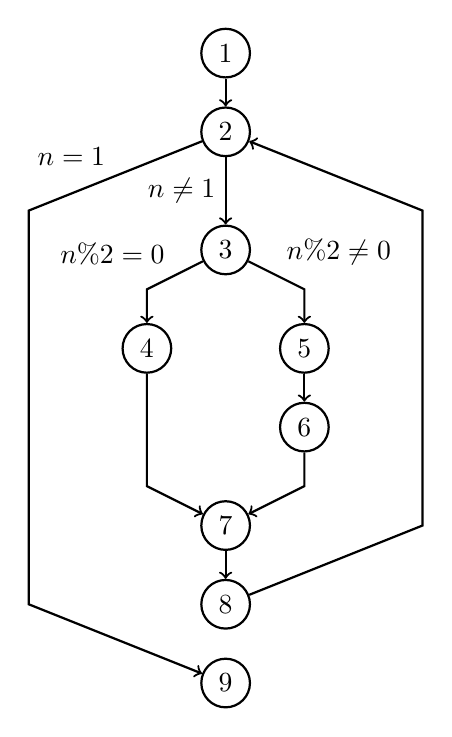
\begin{tikzpicture}
	\node[circle, draw, thick] (n1) at (0, 0) {1};
	\node[circle, draw, thick] (n2) at (0, -1) {2};
	\node[circle, draw, thick] (n3) at (0, -2.5) {3};
	\node[circle, draw, thick] (n4) at (-1, -3.75) {4};
	\node[circle, draw, thick] (n5) at (1, -3.75) {5};
	\node[circle, draw, thick] (n6) at (1, -4.75) {6};
	\node[circle, draw, thick] (n7) at (0, -6) {7};
	\node[circle, draw, thick] (n8) at (0, -7) {8};
	\node[circle, draw, thick] (n9) at (0, -8) {9};

	\draw[->,thick] (n1) -- (n2);
	\draw[->,thick] (n2) -- (n3) node[midway,anchor=east] {$n\ne1$};
	\draw[->,thick] (n2) -- (-2.5,-2) node[midway,anchor=south east,fill=white] {$n=1$} -- (-2.5,-7) -- (n9);
	\draw[->,thick] (n3) -- (-1,-3) node[midway,anchor=south east,fill=white] {$n\%2=0$} -- (n4);
	\draw[->,thick] (n3) -- (1,-3)node[midway,anchor=south west,fill=white] {$n\%2\ne0$} -- (n5);
	\draw[->,thick] (n5) -- (n6);
	\draw[->,thick] (n4) -- (-1,-5.5) -- (n7);
	\draw[->,thick] (n6) -- (1,-5.5) -- (n7);
	\draw[->,thick] (n7) -- (n8);
	\draw[->,thick] (n8) -- (2.5,-6) -- (2.5,-2) -- (n2);
\end{tikzpicture}
		\caption{\ac{CFG} for \cref{fig:cfg_code}}
		\label{fig:cfg}
	\end{subfigure}
	\caption{Example code of an loop with branching code and its representation as a \ac{CFG} (figure taken from \cite{liCacheModelingRealtime1996}).}
	\label{fig:code_and_cfg}
\end{figure}

When analyzing a given task, a \ac{CFG} is built to represent the execution paths of the task's code, including a task's call graph. The control-flow analysis, previously called \textit{high-level analysis}, attempts to gain as much knowledge about the control flow of a given task by identifying loops and their bounds, flow branches, and function calls. When including information about the data flow of the task, it may be possible to exclude paths from the \ac{CFG} that are infeasible and may not be executed at all, for example, paths with mutually exclusive conditions. 

\Cref{fig:code_and_cfg} illustrates an example code snippet and its corresponding \ac{CFG}. 
The code snippet, shown in \cref{fig:cfg_code}, contains loops and branches that determine the sequence of operations based on the value of the variable \texttt{k}. 
The \ac{CFG}, depicted in \cref{fig:cfg}, visually represents the basic blocks of the piece of code, highlighting the possible execution paths.
On base of the \ac{CFG} and some additional information, like the loop bound of $k<10$ in this example, it is possible to deduct constraints describing the flow of the code enabling an estimation of the costs of different execution paths through the graph\cite{liCacheModelingRealtime1996,wilhelmWorstcaseExecutiontimeProblem2008}.
This technique is called \ac{IPET}\cite{wilhelmWorstcaseExecutiontimeProblem2008}.

\subsection{Data Flow Analysis}\label{sec:dfa}
\ac{DFA} is used to analyse the flow of data in a program to detect dependencies and bottlenecks.
Some bottlenecks may be cache misses, e.g., because an \ac{LRU} entry got overwritten. 
Cache misses can significantly impact the execution time of a task, as accessing data from the main memory is much slower compared to accessing it from the cache\cite{liCacheModelingRealtime1996}. 
This can lead to increased execution times and variability in the timing behavior of tasks.
For this reason it is of interest to depict the cache's status to know if the data access results in a cache miss or a cache hit.

\todo{timing accidents - Chen 04 10/53}

Static analysis is advantageous because it does not require actual execution of the code, making it suitable for early stages of development. However, it can be overly conservative, leading to pessimistic WCET estimates due to the need to account for all possible execution paths and hardware behaviors.

\subsection{Measurement-based Analysis}\label{sec:measurement_analysis}
Measurement-based analysis involves executing the code on the target hardware and measuring the execution times to determine the \ac{wcet}. 
This approach relies on collecting empirical data from actual runs of the system, which can provide more accurate and realistic estimates of execution times compared to purely static methods. 
By running the code under various conditions and workloads, measurement-based analysis can capture the dynamic behavior of the system, including the effects of caches, pipelines, and other hardware features that may impact execution time.
However, this method requires a comprehensive set of test cases to ensure that all possible execution paths are covered, which can be challenging and time-consuming\cite{wilhelmWorstcaseExecutiontimeProblem2008}.

One of the main advantages of measurement-based analysis is its ability to provide precise timing information that reflects the actual performance of the system. 
This is particularly useful for complex systems where static analysis may be overly conservative and result in pessimistic WCET estimates.
However, measurement-based analysis also has limitations, such as the difficulty in guaranteeing that the worst-case scenario has been observed during testing. 
Additionally, this approach may not be suitable for early stages of development when the hardware is not yet available, in which case appropriate simulators are used trying to mimic real hardware.\cite{wilhelmWorstcaseExecutiontimeProblem2008}
To address these challenges, hybrid approaches that combine measurement-based and static analysis techniques are often employed to achieve more accurate and reliable WCET estimates\cite{kelterWCETAnalysisOptimization}.

Early flowcharts and \ac{AI}s described by \textcite{cousotAbstractInterpretationUnified1977}

\todo{cache misses}
\todo{overestimation \& pessimism}

\begin{figure}[htbp]
	\centering
	\resizebox{\textwidth}{!}{
		\begin{tikzpicture}
	% Axes
	\draw[->,thick] (0,0) -- (20,0) node[below,anchor=north east]{time};
	\draw[->,thick] (0,0) -- (0,5.5) node[left,rotate=90,anchor=south east]{distribution of times};

	% Execution time distribution (just shape some)
	\draw[thick, fill=black!60, pattern=dots] plot[smooth] coordinates {
	(1,0)
	(2,1)
	(3,1.4)
	(4,3.75)
	(5,3.2)
	(6,1.1)
	(7,2.2)
	(8,0.3)
	(9,0.25)
	(10,0.8)
	(11,0.12)
	(12,0.25)
	(13,0)
	} -- (13,0) -- cycle;
	\draw[thick, fill=black!60, pattern=dots] plot[smooth] coordinates {
	(15,0)
	(16,0.3)
	(16.7,0.3)
	(17,0)
	} -- (17,0) -- cycle;
		% measured times
	\draw[thick, fill=black!30, pattern=crosshatch] plot[smooth] coordinates {
	(3,0)
	(4,2.5)
	(5,1.4)
	(6,0.6)
	(7,1.3)
	(8,0.1)
	(9,0.08)
	(10,0.6)
	(11,0.03)
	} -- (11,0) -- cycle;

	% Vertical markers for BCET, min/max observed times, WCET
	\draw[] (0.5,-1.75) -- (0.5,5.5);
	\node[above,fill=white,align=center,rotate=90,anchor=center] at (0.5,2) {Lower bound};
	\draw[] (1,-1.25) -- (1,5.5);
	\node[above,fill=white,align=center,rotate=90,anchor=center] at (1,2) {BCET};
	\draw[] (3,-0.75) -- (3,5.5);
	\node[above,fill=white,align=center] at (3,5) {Minimal\\observed\\execution\\time};
	\draw[] (11,-0.75) -- (11,5.5);
	\node[above,fill=white,align=center] at (11,5) {Maximal\\observed\\execution\\time};
	\draw[] (17,-1.25) -- (17,5.5);
	\node[above,fill=white,align=center,rotate=90,anchor=center] at (17,2) {WCET};
	\draw[] (19,-1.75) -- (19,5.5);
	\node[above,fill=white,align=center,rotate=90,anchor=center] at (19,2) {Upper bound};

	% Horizontal worst-case performance and guarantee
	\draw[line width=0.7mm,->] (0,4.85) -- (14,4.85) node[midway,above]{worst-case performance} -- (17,4.85);
	\draw[line width=0.7mm,->] (0,4.15) -- (14,4.15) node[midway,above]{worst-case guarantee} -- (19,4.15);

	% Execution time arrows
	\draw[<->] (3,-0.5) -- (11,-0.5) node[midway,fill=white]{measured execution times};
	\draw[<->] (1,-1) -- (3,-1) -- (11,-1) node[midway,fill=white]{possible execution times} -- (17,-1);
	\draw[<->] (0.5,-1.5) -- (3,-1.5) -- (11,-1.5) node[midway,fill=white]{timing predictability} -- (19,-1.5);

	% Annotations
	\draw[->, thick] (13,3) -- (15.9,0.7);  
		\node[draw, fill=white, align=center] at (13,3) {The actual WCET\\ must be found or\\ upper bounded};
	
\end{tikzpicture}
	}
	\caption{
		The graph above illustrates two curves representing the basic concepts of timing analysis.
		The first curve, with the dotted area, shows the range of all possible execution times, with the minimum and maximum values being the \ac{BCET} and \ac{WCET}, respectively.
		The second curve, with the crosshatched area, represents the range of execution times identified through analysis, with the minimum and maximum values being the \textit{minimal observed execution time} and \textit{maximal observed execution time}.
		This graph is adapted from \textcite{wilhelmWorstcaseExecutiontimeProblem2008}.
	}
	\label{fig:overestimation}
\end{figure}

\textcite{kelterWCETAnalysisOptimization} mentions several techniques that can be used for \ac{WCET} analysis, including static analysis, measurement-based analysis, statistical analysis and hybrid approaches.
Static analysis involves analyzing the code without executing it, while measurement-based analysis involves running the code on the target hardware and measuring the execution times.
Hybrid approaches combine both static and measurement-based techniques to provide more accurate \ac{WCET} estimates.

Static analysis is a proper and safe way to get information about the execution times, since it is unhinged from hardware constraints and derived from a meta model created from reviewing the code \cite{kelterWCETAnalysisOptimization}.

To evaluate analysis techniques benchmarks play a significant role.
Providing multiple task sets with known execution scenarios and the tasks behavior the analysis techniques can be tested for its effectiveness. 
Benchmarks commonly used are for example the Mälardalen \ac{WCET} benchmark and the TACLeBench benchmark suite\cite{falkTACLeBenchBenchmarkCollection2016}.

Accurate \ac{WCET} analysis is critical for the design and verification of real-time systems, ensuring that all tasks can be scheduled and executed within their deadlines, thereby maintaining the system's overall reliability and performance\cite{kelterWCETAnalysisOptimization}.
\textcite{kelterWCETAnalysisOptimization} states further that \ac{WCET} analyses are no longer sufficient for newer and complex systems and need to analyze delays and preemptions between tasks as well, resulting in \ac{WCRT}.

\subsection{Critical Instant Theorem}\label{sec:critical_instant_theorem}
The Critical Instant Theorem, introduced by \textcite{liuSchedulingAlgorithmsMultiprogramming1973}, states that the \ac{WCRT} of a task occurs when it is released simultaneously with all higher-priority tasks.
This theorem is fundamental in fixed-priority scheduling, as it helps in determining the worst-case scenario for task execution.

According to the theorem, to find the worst-case response time of a task, one must consider the scenario where the task is released at the same time as all higher-priority tasks. 
This situation is known as the critical instant. By analyzing the system under this condition, one can ensure that the calculated response times are indeed the worst-case values.

The theorem is particularly useful in the context of \ac{RMS} and other fixed-priority scheduling algorithms, as it provides a systematic way to evaluate the schedulability of tasks. 
If all tasks meet their deadlines under the critical instant scenario, the system is considered schedulable.

\subsection{Related Work}\label{sec:related_work}
In the past multiple ideas were presented how to handle or generate task-sets in real-time systems.
A short list of related work is presented in the \cref{sec:related_work:1,sec:related_work:2,sec:related_work:3}

\subsubsection{Assignment and Scheduling Communicating Periodic Tasks in Distributed Real-Time Systems}\label{sec:related_work:1}
\textcite{dar-tzenpengAssignmentSchedulingCommunicating1997} presented a solution to build a task-set with inter-task communication in mind while minimizing the system hazard.
The system hazard is represented by a normalized value of the the maximum task response time.

To tackle the problem they used a task-set with harmonic, periodic tasks and introduced aperiodic tasks as a way to emulate stimuli presented by the systems environment.
The aperiodic tasks were migrated into the periodic harmony by using deferrable servers.

Making use of a search-tree they reduced the complexity of the problem of task allocation to a manageable amount.
The idea is to utilize the tree to run their developed \textit{branch-and-bound technique} to prune the tree of infeasbile paths and task combinations.

\subsubsection{SysWCET\: Whole-System Response-Time Analysis for Fixed-Priority Real-Time Systems}\label{sec:related_work:2}
With \textit{SysWCET} \textcite{dietrichSysWCETWholeSystemResponseTime} explored the idea of mapping out the global control flow into a \textit{system-wide control flow graph} to gain knowledge about the effects of system calls by the presented tasks and reduce the pessimism that often is present when estimating this effects.

To derive actual timing implications, the authors of the paper used the \textit{implicit path enumeration technique} to convert the previously built \ac{CFG} into a \ac{ILP} to solve.
With this the upper bounds of the \ac{WCET} can be derived.

\subsubsection{GenE: A Benchmark Generator for WCET Analysis}\label{sec:related_work:3}
\textcite{wagemannGenEBenchmarkGenerator2015} presented with \textit{GenE} a code generator that bases on the idea to dynamically create benchmarks with known flow facts.

GenE uses patterns to create tasks with a focus on realistic control flows.
These patterns woven together produce control flows with different aspects like assignments, loops and branches.
Knowing these flow facts is big help for improving the analysis that is evaluated with the generated benchmarks.
The benchmarks' code is created by utilizing the Low Level Virtual Machine with its intermediate representation (LLVM-IR).